%
% main.tex
%

% notes = hide | show | only
\documentclass[xcolor=dvipsnames,dvip,notes=show,table]{beamer}

% Para crear una versión 'handout' (impresa)
%\documentclass[xcolor=pst,dvips,handout,notes=show]{beamer}

%
% cabeceras.tex
%

%\usepackage[T1]{fontenc}

\definecolor{ZurichBlue}{rgb}{.255,.41,.884}

\beamertemplateshadingbackground{white!10}{white!10}

\usepackage{beamerthemeWarsaw}
\usepackage{longtable}

%\usecolortheme[named=OliveGreen]{structure} 
\setbeamertemplate{items}[ball] 
\setbeamertemplate{blocks}[rounded][shadow=true] 
\setbeamertemplate{footline}[page number]
\addtocounter{framenumber}{-1}
%Handout
%\usepackage{handoutWithNotes}
%\usepackage{tikz,times}
%\pgfpagesuselayout{2 on 1 with notes}[a4paper,border shrink=5mm]

\usepackage{beamerthemeshadow}
 \useoutertheme[hooks]{tree}
 
% \setbeamertemplate{headline}[default] % The default is just an empty headline.
% \setbeamertemplate{headline}[infolines theme]
% \setbeamertemplate{headline}[miniframes theme]
% \setbeamertemplate{headline}[sidebar theme]
% \setbeamertemplate{headline}[smoothtree theme]
% \setbeamertemplate{headline}[smoothbars theme]
% \setbeamertemplate{headline}[tree]
\beamertemplatetransparentcovereddynamic

% spanish
\usepackage[english]{babel}
\usepackage[utf8]{inputenc}

% diagramas
%\usepackage{pst-eps,epstopdf}
\usepackage{pst-node}
%\usepackage{pst-all}
\usepackage{pst-blur}
%\usepackage{pst-tree}

% incrustaciones de código fuente
\usepackage{listings}

% matemáticas y símbolos
\usepackage{amsmath}
\usepackage{amssymb}
\usepackage[right]{eurosym}
\usepackage{ulem}

% colores
\usepackage{colortbl}

%\usepackage{algorithm2e}
%\usepackage{algorithm}
%\usepackage{algorithmic}


\lstset{%
  language=Python,
	basicstyle=\footnotesize\sffamily,
	keywordstyle=\color{darkred},
 	stringstyle=\color{violet},
 	commentstyle=\color{blue},
 	showspaces=false,
 	showtabs=false,
 	showstringspaces=false,
 	frame=trBL,
        frameround=tttt,
       % backgroundcolor=\color{lightyellow},
 	extendedchars=true,
 	numbers=none,
        aboveskip=0.5cm,
        belowskip=0.5cm,
        xleftmargin=1cm,
        xrightmargin=1cm,
	breaklines=true
}
\definecolor{darkred}{rgb}{0.5, 0, 0}
\definecolor{violet}{rgb}{1, 0, 1}
\definecolor{lightyellow}{rgb}{1,1,0.8}


\usepackage{latexsym}
\usepackage{amsmath}
\usepackage{amssymb}
\usepackage{amsthm}

\usepackage{xspace}

\newcommand{\si}{$\oplus$\xspace}
\newcommand{\no}{$\ominus$\xspace}
\newcommand{\na}{$\odot$\xspace}

%Extraer
\newcommand{\linkeddata}{\textit{Linked Data}\xspace}
\newcommand{\opendata}{\textit{Open Data}\xspace}
\newcommand{\lod}{\textit{Linking Open Data}\xspace}
\newcommand{\ogd}{\textit{Open Government Data}\xspace}
\newcommand{\datasets}{\textit{datasets}\xspace}
\newcommand{\dataset}{\textit{dataset}\xspace}
\newcommand{\provenance}{\textit{provenance}\xspace}
\newcommand{\trust}{\textit{trust}\xspace}
\newcommand{\egov}{\textit{e-government}\xspace}
\newcommand{\pusi}{\textit{Public Sector Information}\xspace}
\newcommand{\gd}{\textit{Government Data}\xspace}
\newcommand{\wod}{Web de Datos\xspace}
\newcommand{\wode}{\textit{Web of Data}\xspace}
\newcommand{\eproc}{\textit{e-Procurement}\xspace}
\newcommand{\gld}{\textit{Government Linked Data}\xspace}

\hyphenation{real}

\newrgbcolor{ColorEncabezadoTabla}{0.7 0.7 0.9}
\newrgbcolor{ColorFila1}{0.8 0.8 0.7}
\newrgbcolor{ColorFila2}{0.8 0.7 0.8}
\newrgbcolor{ColorTotal}{0.7 0.9 0.7}


% \usepackage{tikz,times}
% \usetikzlibrary{mindmap,backgrounds}




%%%%%%%%%%%%%%%%%%%%%%%%%%%%%%%%%%%%%%%%%%%%%%%%%%%%%%%%%%%%%%%%%%%%%%

\title[MapReduce Intro]{Evaluation of the Map Reduce Programming Model}
\author[Dr. Jose María Álvarez Rodríguez]{\textbf{Introduction and Examples}\\ \vspace{0.3cm} Dr. Jose María Álvarez Rodríguez \\ \vspace{0.3cm} ``Quality Management in Service-based Systems and Cloud Applications'' \\ \vspace{0.3cm} FP7 RELATE-ITN}
\subtitle{}
\institute{South East European Research Center}


\date{Thessaloniki, 20th of April, 2013}

\begin{document}

\frame{
\titlepage

}

\frame{
\tableofcontents

}


%%%%%%%%%%%%%%%%%%%%%%%%%%%%%%%%%%%%%%%%%%%%%%%%%%%%%%%%%%%%%%%%%%%%%%
\section{MapReduce in a nutshell}


\frame{
  \frametitle{Features}

\begin{block}{A programming model...}
\begin{enumerate}
 \item Large-scale distributed data processing
 \item Simple but restricted
 \item Paralell programming
 \item Extensible
\end{enumerate}
\end{block}

}


\begin{frame}[fragile]
  \frametitle{Antecedents}

\begin{alertblock}{Functional programming}
\begin{enumerate}
 \item Inspired
 \item ...but not equivalent
\end{enumerate}
\end{alertblock}

\begin{exampleblock}{Example in Python}
``Given a list of numbers between 1 and 50 print only even numbers''
\begin{lstlisting}
print filter(lambda x: x % 2 == 0, range(1, 50))
\end{lstlisting}
\end{exampleblock}
\begin{itemize}
 \item A list of numbers (data)
 \item A condition (even numbers)
 \item A function \textit{filter} that is applied to the list (map)
\end{itemize}


\end{frame}


\begin{frame}[fragile]
  \frametitle{...Other examples...}

\begin{exampleblock}{Example in Python}
``Return the sum of the squares of a list of numbers between 1 and 50''
\begin{lstlisting}
import operator
reduce(operator.add, map((lambda x: x **2), range(1,50)) , 0)
\end{lstlisting}
\end{exampleblock}

\begin{itemize}
 \item ``reduce'' is equivalent to ``foldl'' in other func. languages as Haskell
 \item other math considerations should be taken into account (kind of operator)...
\end{itemize}


\end{frame}


\frame{
  \frametitle{Some interesting points...}

\begin{alertblock}{The Map Reduce framework...}
\begin{enumerate}
 \item Inspired in functional programming concepts (\textbf{but not equivalent})
 \item Problems that can be paralellized
 \item Sometimes recursive solutions
 \item ...
\end{enumerate}
\end{alertblock}

}

\frame{
  \frametitle{Basic Model}
\begin{figure}[!htb]
\centering
 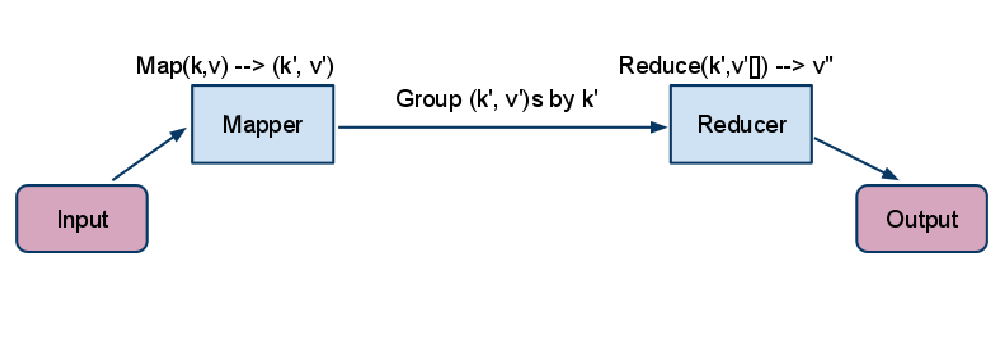
\includegraphics[width=7cm]{img/basic-model-mapreduce}
\end{figure}

\tiny
``MapReduce: The Programming Model and Practice'', SIGMETRICS, Turorials 2009, Google.
}






\frame{
  \frametitle{Tip}
\begin{exampleblock}{What is MapReduce?}
It is a \textbf{framework} inspired in \textbf{functional programming} to tackle problems in which steps 
can be \textbf{paralellized} applying a \textbf{divide and conquer} approach.
\end{exampleblock}

}

\section{Thinking in MapReduce}

\frame{
  \frametitle{When should I use MapReduce?}
\begin{exampleblock}{Query}
\begin{itemize}
 \item Index and Search: inverted index
 \item Filtering
 \item Classification 
 \item Recommendations: clustering or collaborative filtering
\end{itemize}
\end{exampleblock}

\begin{block}{Analytics}
\begin{itemize}
 \item Summarization and statistics
 \item Sorting and merging 
 \item Frequency distribution
 \item SQL-based queries: group-by, having, etc.
 \item Generation of graphics: histograms, scatter plots.
\end{itemize}

\end{block}

}


\frame{
  \frametitle{How Google uses MapReduce (80\% of data processing)...}

\begin{itemize}
\item Large-scale web search indexing
\item Clustering problems for Google News
\item Produce reports for popular queries, e.g. Google Trend
\item Processing of satellite imagery data
\item Language model processing for statistical machine translation
\item Large-scale machine learning problems
\item \ldots
\end{itemize}


}

\frame{
  \frametitle{Comparison of MapReduce and other approaches}
\begin{figure}[!htb]
\centering
 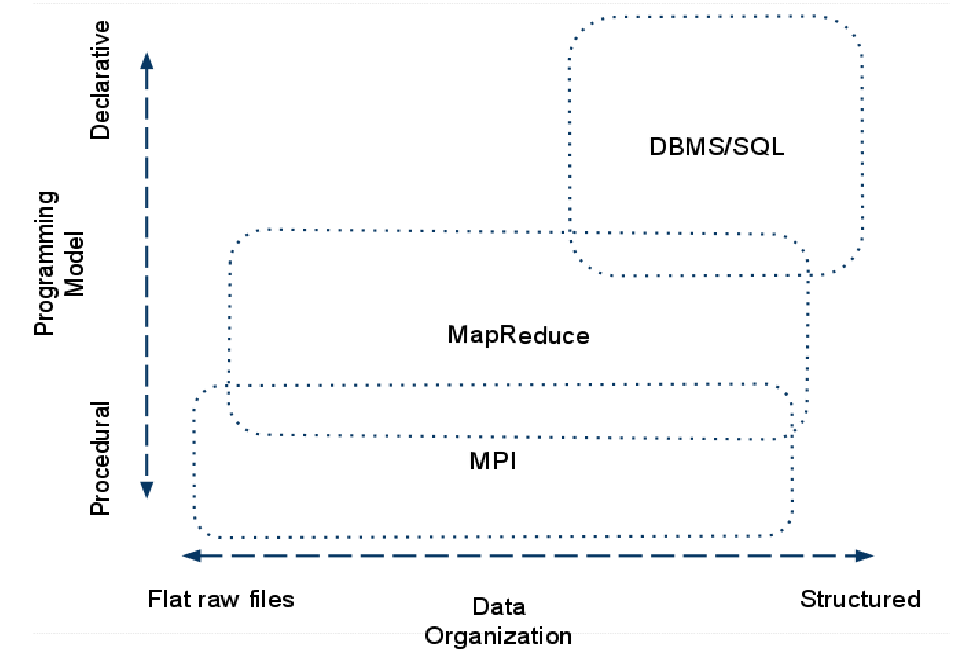
\includegraphics[width=8cm]{img/comparison-map-reduce}
\end{figure}

\tiny
``MapReduce: The Programming Model and Practice'', SIGMETRICS, Turorials 2009, Google.

}

\frame{
  \frametitle{Evaluation of MapReduce and other approaches}
\begin{figure}[!htb]
\centering
 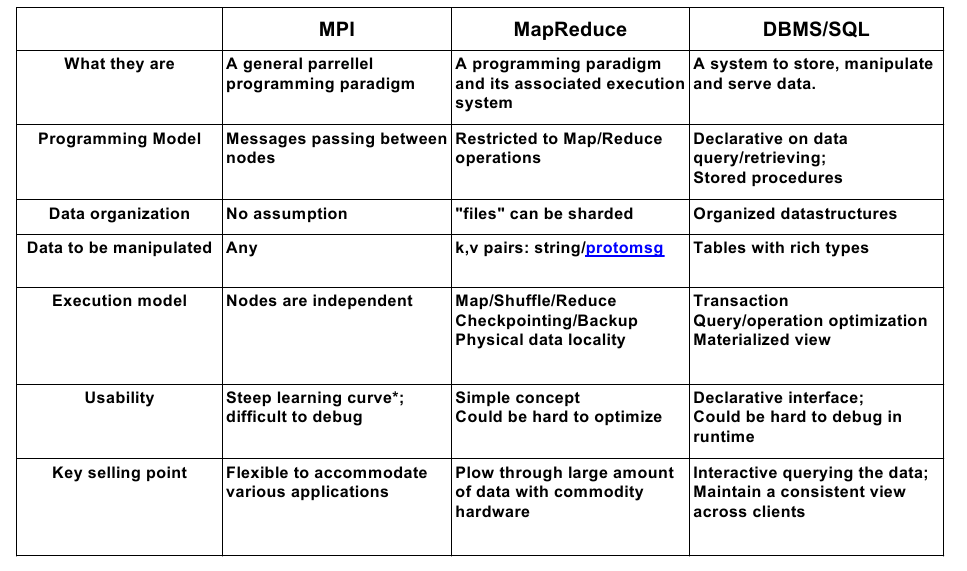
\includegraphics[width=8cm]{img/table-features}
\end{figure}

\tiny
``MapReduce: The Programming Model and Practice'', SIGMETRICS, Turorials 2009, Google.

}


\frame{
  \frametitle{Tip}
\begin{exampleblock}{What can I do in MapReduce?}

\end{exampleblock}

}

\section{Applying MapReduce}


\frame{
  \frametitle{Tip}
\begin{exampleblock}{How can I use MapReduce ?}

\end{exampleblock}

}


\section{Implementing MapReduce algorithms}


\frame{
  \frametitle{Tip}
\begin{exampleblock}{How can I run a MapReduce framework?}

\end{exampleblock}

}

\section{Success Stories with MapReduce}


\frame{
  \frametitle{Tip}
\begin{exampleblock}{Who is using MapReduce?}

\end{exampleblock}

}

\section{Beyond MapReduce}


\frame{
  \frametitle{Tip}
\begin{exampleblock}{What's next?}

\end{exampleblock}

}


\section{Summary}

\frame{


}




\section{Conclusions}

\frame{
\titlepage

}



\section{Future Work}

\frame{
\titlepage

}



\nocite{*}
% \section*{Acknowledgements}
% \frame{
%   \frametitle{All have contributed...} 
% \begin{figure}[!htb]
% \centering
%  \includegraphics[width=9cm]{imgs/linkedin}
% \end{figure}
% }

%%%%%%%%%%%%%%%%%%%%%%%%%%%%%%%%%%%%%%%%%%%%%%%%%%%%%%%%%%%%%%%%%%%%%%
\appendix
\section*{References}
\bibliographystyle{abbrv}
\bibliography{references}
% 
% 
%\section*{Preguntas}
% \input{preguntas-preparadas}


\end{document}

